\documentclass[10pt,a4paper]{article}
\usepackage{graphicx, wrapfig, palatino, subfigure, multirow, comment}
\usepackage{enumerate}
\usepackage{color}
\usepackage{hyperref}
\usepackage[cm]{fullpage}

\renewcommand\thefigure{R-\arabic{figure}}

\pagestyle{empty}
\usepackage{setspace} 
\usepackage{anysize,amsmath,amssymb}
\usepackage[cm]{fullpage}
\marginsize{1.0in}{1.0in}{0.8in}{0.8in}






\begin{document}
\title{Paper Reading 2 of CS211 in Fall 2022}
\author{Anonymous}
\date{}
\maketitle


\section{Paper}
A. Ros and S. Kaxiras, "Speculative Enforcement of Store Atomicity," 2020 53rd Annual IEEE/ACM International Symposium on Microarchitecture (MICRO), 2020, pp. 555-567, doi: 10.1109/MICRO50266.2020.00053.

\section{Problem and Theory Solution}
\begin{center}
	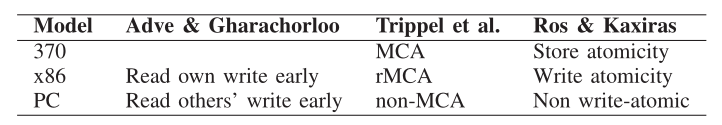
\includegraphics[scale = 0.4]{1.png}
\end{center}
These are current memory consistency model implementations, X86-TSO: a core see its own stores before other cores, while IBM 370 all cores see all stores atomically, x86-TSO is less intuitive than IBM 370, the author want to have a more stricter, more readable and more intuitive solution. \\
The author believed that a load performed by a forwarding from an $in-limbo$ store is not speculative, younger loads performed after that forwarding are. The author put up with a idea that they only perform dynamically enforcement of store atomicity only when the detection of its violation occurs.

\section{Background of X86 Non-store-atmoic Semantics}
\subsection{Ordered Stores}
Load a value will not be performed until store the same value is inserted in the memory order and all cores can see the new value, preventing loads seeing different store orders.
\subsection{Independent Stores}
Load value x in one core and load value y in another core will not be able perform until the respective stores in the two cores are written from the store buffers to the L1s and hence inserted in the memory order. Here is three possible situations and one impossible situation.
\begin{center}
	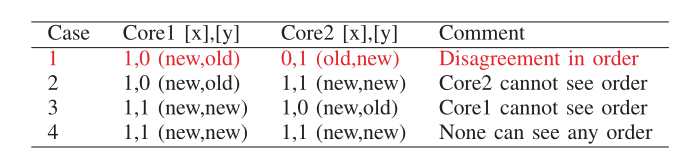
\includegraphics[scale = 0.4]{2.png}
\end{center}  
If one of the cores is able to discern an order between the two independent stores, then another core cannot, that is, there is no disagreement about the order of independent stores in a store-atomic implementation.

\section{Speculative Enforcement of Store Atomicity}
Two solutions to guarantee store atomicity are
\begin{itemize}
	\item  Prevent the consumer load of the store-to-load forwarding, from being performed until store is inserted in memory order.
	\item Treat load as speculative, not allowing it to retire until the store buffer empties.
\end{itemize}
They both highly effect performance.\\
The author will make load value y in core 1 speculative until store x is ordered. If an invalidation is received for y in the interim, it must squash load y and re-excute it. The author's implementation is base on SLF loads, that is, an SLF(Store-to-Load-Forwarded) load establishes a connection between a store in the store buffer and a "retire gate" at the head of the load queue, to prevent the retirement of any younger SA-speculative loads until the store is inserted in memory order. 
\begin{center}
	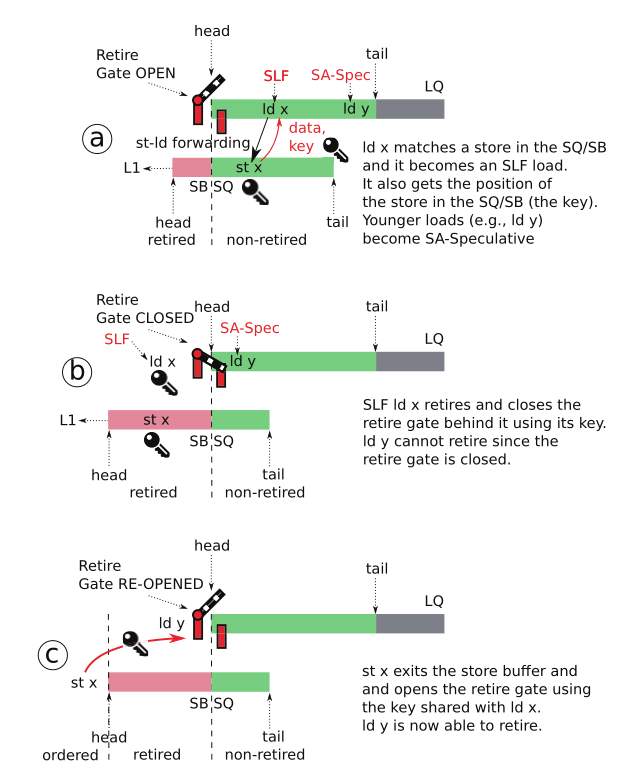
\includegraphics[scale = 0.4]{3.png}
\end{center} 
\begin{itemize}
	\item  \textbf{Step 1: } Setting SLF loads on store-to-load forwarding, the load receives its value and is marked as an SLF and keeps a pointer to the position of the store in the SB.
	\item\textbf{Step 2: } Closing the retire gate, if the load has the valid key of the older store, the retire gate is closed by the key of the load, preventing younger SA-speculative loads from retiring.
	\item \textbf{Step 3: } Reopening the retire gate, if the key of the store matches the key(closed the door), then the retire gate is reopened.
\end{itemize}
In summary, \textbf{By marking the load queue and prevent load operations to commit, it can stall loads in the reorder buffer until the store that forwards value to load commit.}


\section{Evaluation Environment}
\textbf{Sniper} with in-house processor model and \textbf{GEMS} 
\begin{itemize}
	\item Reorder buffer: 224 entries
	\item SB: 56 entries
	\item Load queue: 72 entries
	\item Processor: 8 out-of-order Intel Skylake cores
\end{itemize}
For parallel benchmark, using \textbf{Splash-3} and \textbf{Parsec-3.0}.\\
For sequential benchmark, using \textbf{SPEC CPU 2017}.

\section{Results and Conclusion}
The author get an efficient implementation of the IBM 370 model with similar performance(+2.7\% performance) (<3\% overhead) than x86-TSO at a low complexity and hardware cost. 

\section{Thinking and Questions}
\begin{itemize}
	\item For multiple store-forward-loads on different addresses, is it possible for each SFL start a new gate or the later loads is treated as speculative?
	\item Since it do not have very significant performance improvement compared with stalling the forwarding load, it might caused by overlappings between the draining of  the store buffer and the execution of the next load.
\end{itemize}



\begin{comment}
{
	\bibliographystyle{unsrt}	
	\bibliography{papers} % Make sure your bib file name is papers.bib.
}
\end{comment}

\end{document}
